\chapter{LNAs Control Board}

\section{Introduzione}

Questo documento descrive brevemente il controllo dei ricevitori mediante le schede 
progettate e realizzate a Medicina. Ogni ricevitore ospiter\`a due schede, una per
il \textbf{controllo del dewar} e una per il \textbf{controllo degli LNA}.

Il protocollo di comunicazione con le schede a microcontrollore \`e descritto nel documento interno 
IRA n.358/04 (F.Fiocchi, G.Macaferri, A.Oralti, M.Morsiani), il firmware \`e stato 
realizzato da Franco Fiocchi mentre dell'hardware se ne sono occupati Sandro Cattani
ed Andrea Maccaferri.

La libreria che permette di comunicare ad alto livello con le schede \`e stata realizzata da Marco Buttu
ed Andrea Orlati, ed \`e articolata su due livelli indipendenti: un primo livello che fornisce
un'interfaccia per la comunicazione con le schede (sostanziamente un'implementazione del protocollo di
comunicazione), ed un secondo e pi\`u alto livello che mediante l'utilizzo della prima libreria definisce
una interfaccia per la comunicazione con il ricevitore.

In questo documento descriveremo solo l'architettura della scheda per il controllo degli LNA, poich\`e per
questa non \`e semplice comprenderne il funzionamento e documentare il codice senza l'ausilio di
uno schema a blocchi.

\section{LNAs control board: schema a blocchi dell'hardware}
La scheda per il controllo degli LNA permette di leggere i valori delle grandezze
$V_D$, $I_D$ e $V_G$ di ogni stadio degli LNA di ciascun feed, e per ogni canale.
Queste letture vengono fatte sulla porta AD24. Ogni lettura consente di recuperare i valori delle grandezze
di 8 canali (4 feed, 2 canali per feed). Per poter effettuare una lettura \`e necessario indicare
quali grandezze andare a leggere, e questo viene fatto andando a scrivere sulla porta DIO. Le porte di nostro
interesse quindi sono due:
\begin{itemize}
\item DIO: \`e una porta a 16 bit accessibile in lettura/scrittura;
\item AD24: \`e una porta con 8 locazioni da 32 bit (4 byte per ogni locazione).
\end{itemize}
Iniziamo con la descrizionie della porta AD24, schematizzata in figura~\ref{fig:AD24}.
\begin{center}
\begin{figure}[!htbp]
        \begin{center}
        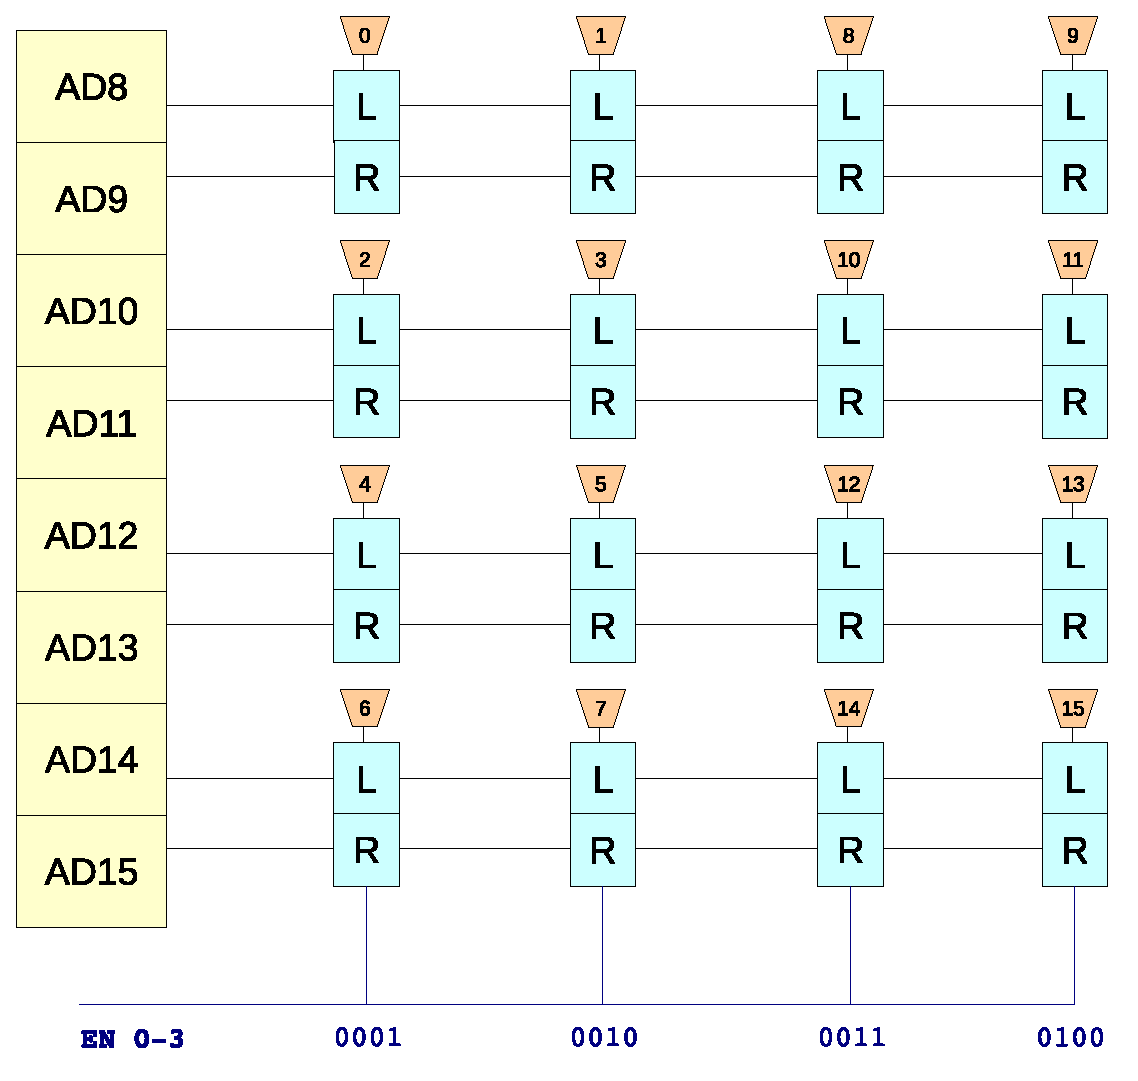
\includegraphics[width=11cm]{figure/AD24}
        \end{center}
        \figurecaption{Schema a blocchi della porta AD24}
         \label{fig:AD24}
\end{figure}
\end{center}
Una lettura dalla porta AD24 fornisce un dato composto da 32 byte (ogni locazione $AD8, \dots, AD15$
\`e composta da 4 byte). Dalla locazione AD8 sar\`a possibile leggere le grandezze di interesse per il 
canale left di uno dei seguenti feed: 0, 1, 8 o 9, mentre dalla locazione AD9 sar\`a possibile leggere
i valori del canale right per gli stessi feed, e cos\`i via per tutti gli altri sulla base dello schema
di figura~\ref{fig:AD24}. \`E possibile selezionare i feed su cui andare a leggere impostando sulla porta
DIO il valore di \texttt{EN 0-3}; come si vede in figura il valore \texttt{0001} di \texttt{EN 0-3} permette
di selezionare la prima colonna, il valore \texttt{0010} la seconda e cos\`i via per le altre due. La grandezza
da leggere invece dipende dal valore \texttt{AD 0-3} impostato nel DIO; questo permette di selezionare il valore di
$V_D$, $I_D$ o $V_G$ di uno dei cinque stadi degli LNA. La porta DIO \`e schematizzata in figura~\ref{fig:DIO}.
\begin{center}
\begin{figure}[!htbp]
        \begin{center}
        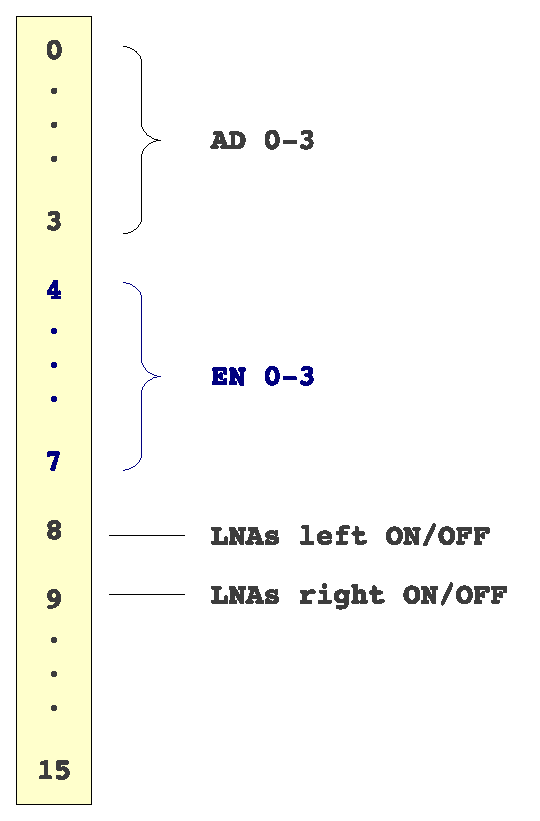
\includegraphics[width=5cm]{figure/DIO}
        \end{center}
        \figurecaption{Schema della porta DIO}
         \label{fig:DIO}
\end{figure}
\end{center}
Nella tabella~\ref{tab:AD03} sono indicati i valori di \texttt{AD 03} da impostare sulla porta DIO
per selezioare la grandezza da leggere.
\renewcommand\arraystretch{1.2}
\begin{table}[!htbp]
\begin{center}
\begin{tabular}{ c | c | p{4cm} }
\texttt{AD 0-3} & \textbf{Segnale} & \textbf{Stadio} \\
\hline 
\hline 
\texttt{0000} & $V_D$ & primo \\
\hline 
\texttt{0001} & $I_D$ & primo \\
\hline 
\texttt{0010} & $V_G$ & primo \\
\hline 
\texttt{0011} & $V_D$ & secondo \\
% \hline 
% \texttt{0100} & $I_D$ & secondo \\
% \hline 
% \texttt{0101} & $V_G$ & secondo \\
% \hline 
\dots & \dots & \dots \\
\hline
% \texttt{0110} & $V_D$ & terzo \\
% \hline 
% \texttt{0111} & $I_D$ & terzo \\
% \hline 
% \texttt{1000} & $V_G$ & terzo \\
% \hline 
% \texttt{1001} & $V_D$ & quarto \\
% \hline 
% \texttt{1010} & $I_D$ & quarto \\
% \hline 
% \texttt{1011} & $V_G$ & quarto \\
% \hline 
% \texttt{1100} & $V_D$ & quinto \\
% \hline 
% \texttt{1101} & $I_D$ & quinto \\
% \hline 
% \texttt{1110} & $V_G$ & quinto \\
% \hline 
\end{tabular}
\caption{Valori di \texttt{AD 0-3} per la selezione della grandezza da leggere}
\label{tab:AD03}
\end{center}
\end{table}

Supponiamo ad esempio di voler leggere gli 8 valori (4 feed, 2 canali per feed) di $V_G$ del terzo 
stadio dei feed 8, 10, 12 e 14. Il valore di \texttt{AD 0-3} sar\`a \texttt{0011} mentre il valore 
di \texttt{EN 0-3} sar\`a \texttt{1000}. Faremo allora due richieste: la prima (\texttt{SET\_DATA}) 
ha lo scopo di configurare la porta DIO in modo da impostare i valori di 
\texttt{AD 0-3} e \texttt{EN 0-3}, mentre la seconda (\texttt{GET\_DATA}) \`e la lettura della 
grandezza richiesta ($V_G$ del terzo stadio per i vari feed):
\begin{itemize}
\item \texttt{SET\_DATA}: avr\`a quattro parametri:
\begin{enumerate}
\item \textbf{data type}: unsigned da 8 bit
\item \textbf{port type}: DIO
\item \textbf{port number}: da 0 a 7 (8 bit, dall'indice 0 all'indice 7)
\item \textbf{value}: \texttt{00111000} (\texttt{AD 0-3} + \texttt{EN 0-3})
\end{enumerate}
\item \texttt{GET\_DATA}: avr\`a tre parametri:
\begin{enumerate}
\item \textbf{data type}: 32 bit floating point
\item \textbf{port type}: AD24
\item \textbf{port number}: da 8 a 15
\end{enumerate}
\end{itemize}
Dopo aver dato il comando \texttt{SET\_DATA} \`e necessario attendere un tempo di guardia prima di
andare a leggere i valori con \texttt{GET\_DATA}, in modo da avere le uscite stabili; questo
tempo di guardia non deve essere inferiore ai $200$\,ms.

Il dato letto con il \texttt{GET\_DATA} \`e un 32 byte, che una volta scomposto in elementi da 4byte ci fornisce
8 valori analogici di tensione, che andranno poi convertiti secondo oppurtune formule di trasformazione.



